%%%%%%%%%%%%%%%%%%%%%%%%%%%%%%%%%%%%%%%%%
% Lachaise Assignment
% LaTeX Template
% Version 1.0 (26/6/2018)
%
% This template originates from:
% http://www.LaTeXTemplates.com
%
% Authors:
% Marion Lachaise & François Févotte
% Vel (vel@LaTeXTemplates.com)
%
% License:
% CC BY-NC-SA 3.0 (http://creativecommons.org/licenses/by-nc-sa/3.0/)
% 
%%%%%%%%%%%%%%%%%%%%%%%%%%%%%%%%%%%%%%%%%

%----------------------------------------------------------------------------------------
%	PACKAGES AND OTHER DOCUMENT CONFIGURATIONS
%----------------------------------------------------------------------------------------

\documentclass{article}

%%%%%%%%%%%%%%%%%%%%%%%%%%%%%%%%%%%%%%%%%
% Lachaise Assignment
% Structure Specification File
% Version 1.0 (26/6/2018)
%
% This template originates from:
% http://www.LaTeXTemplates.com
%
% Authors:
% Marion Lachaise & François Févotte
% Vel (vel@LaTeXTemplates.com)
%
% License:
% CC BY-NC-SA 3.0 (http://creativecommons.org/licenses/by-nc-sa/3.0/)
% 
%%%%%%%%%%%%%%%%%%%%%%%%%%%%%%%%%%%%%%%%%

%----------------------------------------------------------------------------------------
%	PACKAGES AND OTHER DOCUMENT CONFIGURATIONS
%----------------------------------------------------------------------------------------

\usepackage{amsmath,amsfonts,stmaryrd,amssymb} % Math packages

\usepackage{enumerate} % Custom item numbers for enumerations
\usepackage{natbib}
\usepackage[ruled]{algorithm2e} % Algorithms

\usepackage[framemethod=tikz]{mdframed} % Allows defining custom boxed/framed environments

\usepackage{listings} % File listings, with syntax highlighting
\lstset{
	basicstyle=\ttfamily, % Typeset listings in monospace font
}

%----------------------------------------------------------------------------------------
%	DOCUMENT MARGINS
%----------------------------------------------------------------------------------------

\usepackage{geometry} % Required for adjusting page dimensions and margins

\geometry{
	paper=a4paper, % Paper size, change to letterpaper for US letter size
	top=2.5cm, % Top margin
	bottom=3cm, % Bottom margin
	left=2.5cm, % Left margin
	right=2.5cm, % Right margin
	headheight=14pt, % Header height
	footskip=1.5cm, % Space from the bottom margin to the baseline of the footer
	headsep=1.2cm, % Space from the top margin to the baseline of the header
	%showframe, % Uncomment to show how the type block is set on the page
}

%----------------------------------------------------------------------------------------
%	FONTS
%----------------------------------------------------------------------------------------

\usepackage[utf8]{inputenc} % Required for inputting international characters
\usepackage[T1]{fontenc} % Output font encoding for international characters

\usepackage{XCharter} % Use the XCharter fonts

%----------------------------------------------------------------------------------------
%	COMMAND LINE ENVIRONMENT
%----------------------------------------------------------------------------------------

% Usage:
% \begin{commandline}
%	\begin{verbatim}
%		$ ls
%		
%		Applications	Desktop	...
%	\end{verbatim}
% \end{commandline}

\mdfdefinestyle{commandline}{
	leftmargin=10pt,
	rightmargin=10pt,
	innerleftmargin=15pt,
	middlelinecolor=black!50!white,
	middlelinewidth=2pt,
	frametitlerule=false,
	backgroundcolor=black!5!white,
	frametitle={Command Line},
	frametitlefont={\normalfont\sffamily\color{white}\hspace{-1em}},
	frametitlebackgroundcolor=black!50!white,
	nobreak,
}

% Define a custom environment for command-line snapshots
\newenvironment{commandline}{
	\medskip
	\begin{mdframed}[style=commandline]
		}{
	\end{mdframed}
	\medskip
}

%----------------------------------------------------------------------------------------
%	FILE CONTENTS ENVIRONMENT
%----------------------------------------------------------------------------------------

% Usage:
% \begin{file}[optional filename, defaults to "File"]
%	File contents, for example, with a listings environment
% \end{file}

\mdfdefinestyle{file}{
	innertopmargin=1.6\baselineskip,
	innerbottommargin=0.8\baselineskip,
	topline=false, bottomline=false,
	leftline=false, rightline=false,
	leftmargin=2cm,
	rightmargin=2cm,
	singleextra={%
			\draw[fill=black!10!white](P)++(0,-1.2em)rectangle(P-|O);
			\node[anchor=north west]
			at(P-|O){\ttfamily\mdfilename};
			%
			\def\l{3em}
			\draw(O-|P)++(-\l,0)--++(\l,\l)--(P)--(P-|O)--(O)--cycle;
			\draw(O-|P)++(-\l,0)--++(0,\l)--++(\l,0);
		},
	nobreak,
}

% Define a custom environment for file contents
\newenvironment{file}[1][File]{ % Set the default filename to "File"
	\medskip
	\newcommand{\mdfilename}{#1}
	\begin{mdframed}[style=file]
		}{
	\end{mdframed}
	\medskip
}

%----------------------------------------------------------------------------------------
%	NUMBERED QUESTIONS ENVIRONMENT
%----------------------------------------------------------------------------------------

% Usage:
% \begin{question}[optional title]
%	Question contents
% \end{question}

\mdfdefinestyle{question}{
	innertopmargin=1.2\baselineskip,
	innerbottommargin=0.8\baselineskip,
	roundcorner=5pt,
	nobreak,
	singleextra={%
			\draw(P-|O)node[xshift=1em,anchor=west,fill=white,draw,rounded corners=5pt]{%
				Question \theQuestion\questionTitle};
		},
}

\newcounter{Question} % Stores the current question number that gets iterated with each new question

% Define a custom environment for numbered questions
\newenvironment{question}[1][\unskip]{
	\bigskip
	\stepcounter{Question}
	\newcommand{\questionTitle}{~#1}
	\begin{mdframed}[style=question]
		}{
	\end{mdframed}
	\medskip
}

%----------------------------------------------------------------------------------------
%	WARNING TEXT ENVIRONMENT
%----------------------------------------------------------------------------------------

% Usage:
% \begin{warn}[optional title, defaults to "Warning:"]
%	Contents
% \end{warn}

\mdfdefinestyle{warning}{
	topline=false, bottomline=false,
	leftline=false, rightline=false,
	nobreak,
	singleextra={%
			\draw(P-|O)++(-0.5em,0)node(tmp1){};
			\draw(P-|O)++(0.5em,0)node(tmp2){};
			\fill[black,rotate around={45:(P-|O)}](tmp1)rectangle(tmp2);
			\node at(P-|O){\color{white}\scriptsize\bf !};
			\draw[very thick](P-|O)++(0,-1em)--(O);%--(O-|P);
		}
}

% Define a custom environment for warning text
\newenvironment{warn}[1][Warning:]{ % Set the default warning to "Warning:"
	\medskip
	\begin{mdframed}[style=warning]
		\noindent{\textbf{#1}}
		}{
	\end{mdframed}
}

%----------------------------------------------------------------------------------------
%	INFORMATION ENVIRONMENT
%----------------------------------------------------------------------------------------

% Usage:
% \begin{info}[optional title, defaults to "Info:"]
% 	contents
% 	\end{info}

\mdfdefinestyle{info}{%
topline=false, bottomline=false,
leftline=false, rightline=false,
nobreak,
singleextra={%
\fill[black](P-|O)circle[radius=0.4em];
\node at(P-|O){\color{white}\scriptsize\bf i};
\draw[very thick](P-|O)++(0,-0.8em)--(O);%--(O-|P);
}
}

% Define a custom environment for information
\newenvironment{info}[1][Info:]{ % Set the default title to "Info:"
	\medskip
	\begin{mdframed}[style=info]
		\noindent{\textbf{#1}}
		}{
	\end{mdframed}
}
 % Include the file specifying the document structure and custom commands

%----------------------------------------------------------------------------------------
%	ASSIGNMENT INFORMATION
%----------------------------------------------------------------------------------------

\title{Designing a Lap Simulator for the Shell Eco-Marathon} % Title of the assignment

\author{Supervisor: Tim Baker\\Student: Hasha Dar} % Author name and email address

\date{University College London --- \today} % University, school and/or department name(s) and a date

%----------------------------------------------------------------------------------------

\begin{document}

\maketitle % Print the title

%----------------------------------------------------------------------------------------
%	INTRODUCTION
%----------------------------------------------------------------------------------------
\section{Project Background \& Problem}
The Shell Eco-Marathon is a competition at the school and university level for students focusing on energy optimisation in vehicles. The aim of the competition is to develop new innovations in energy efficiency for vehicles on the road with the idea of reducing carbon emissions \citep{ShellEco2021}. I will be focusing on the 'Prototype' category for the competition, which involves designing a hydrogen-powered single-seater vehicle with a focus on attaining ultra-efficiency through the optimisation of the aerodynamic and performance characteristics of the vehicle.

For an ultra-energy-efficient vehicle, there are many sources of inefficiency. Some of them are aerodynamic drag (air resistance), friction drag (from the road surface) and losses in the powertrain (electricity generation, mechanical losses) \citep{Wei2019}. The design itself of the car must be optimised to increase its performance such as the weight of the vehicle \citep{Tsirogiannis2019}.

A problem that arises when investigating and modelling these variables is that there is no way of testing certain performance characteristics within the holistic context of the competition virtually. Currently, to test newly designed components and its overall impact on the performance of the vehicle, the part must be prototyped and installed on the vehicle, and then experimentally tested. This presents a problem as this is costly, time-consuming and constrains the number of prototypes that can be made.

A transient, dynamic lap simulator will allow the analysis of the vehicle's various performance characteristics. This will allow the team to optimise and prototype designs much more effectively. The team would be able to test the vehicle on the final test track, without the cost of being there physically.
\section{Project Aim}
During the design phase of the vehicle, a lot of work must go into modelling performance variables of the vehicle. This may be done through mathematical analysis and through the use of software such as Computational Fluid Dynamics (CFD) and Finite Element Analysis (FEA). These methods allow us to test whether our design meets our performance criteria (in a virtual sense). This project will focus on bringing together the various performance characteristics of the vehicle to be able to analyse the car in a contextual manner. A lap simulator will allow the team to see how their prototype design will function in a real-world scenario, rather than as a discrete set of performance variables. Hence, with a lap simulator the team will be able to:
\begin{itemize}
	\item unify the various computational models that assess parts of the vehicles performance
	\item see where the primary energy inefficiencies are in a transient, dynamics test, allowing targeted improvement of the vehicle's performance
	\item reduce the number of physical tests for the vehicle,
	      \begin{itemize}
		      \item lowering cost
		      \item reducing development time
		      \item minimising the number of prototype parts manufactured
	      \end{itemize}
\end{itemize}
\section{Previous Work, Activities \& Project Potential}
A lot of analysis and papers have been released pertaining to the Shell Eco-marathon competition and the development of its vehicles. \citep{Stabile2021} presents a detailed numerical model of the power demand of a Shell Eco-marathon vehicle. Here, an in-depth analysis of the power demand around the Shell Eco-marathon circuit is discussed.

\citep{Punov2021} also studies energy management strategies and also uses a generic lap simulation to study the power demand. Both of these models "simulate" the lap in a 1-dimensional sense e.g. by analysing throttle input. They also focus on the 'urban concept' category and not the 'prototype' category.

\citep{Dol2016} looks at the development of the vehicle subsystems but does not simulate each part within the wider context of the vehicle. Analysis on individual components is thorough but a simulation of the full vehicle or its competition environment is neglected.

\citep{Wei2019} also looks at the powertrain efficiency of the vehicle around a specific test track, however only two cases are considered in their transient test, idealising the testing conditions.

This project has the potential of forming part of a wider vehicle development strategy platform, allowing teams to look at their cars in the virtual world and see how they would stack up around a real test track. The modelling of the various performance parameters on a transient, dynamic test track will allow teams to better understand which parameters have the most effect on the performance of the vehicle.
\section{Budget}
The project will be utilising software and resources from the Mechanical Engineering department which may be used for free. There are no foreseeable costs for the project.
\section{Declaration}
\begin{quote}
	\textit{I, Hasha Dar, confirm that the work presented in this report is my own. Where information has been derived from	other sources, I confirm that this has been indicated in the report.}
\end{quote}
\section{Gantt Chart}
\begin{figure}[h]
	\centering
	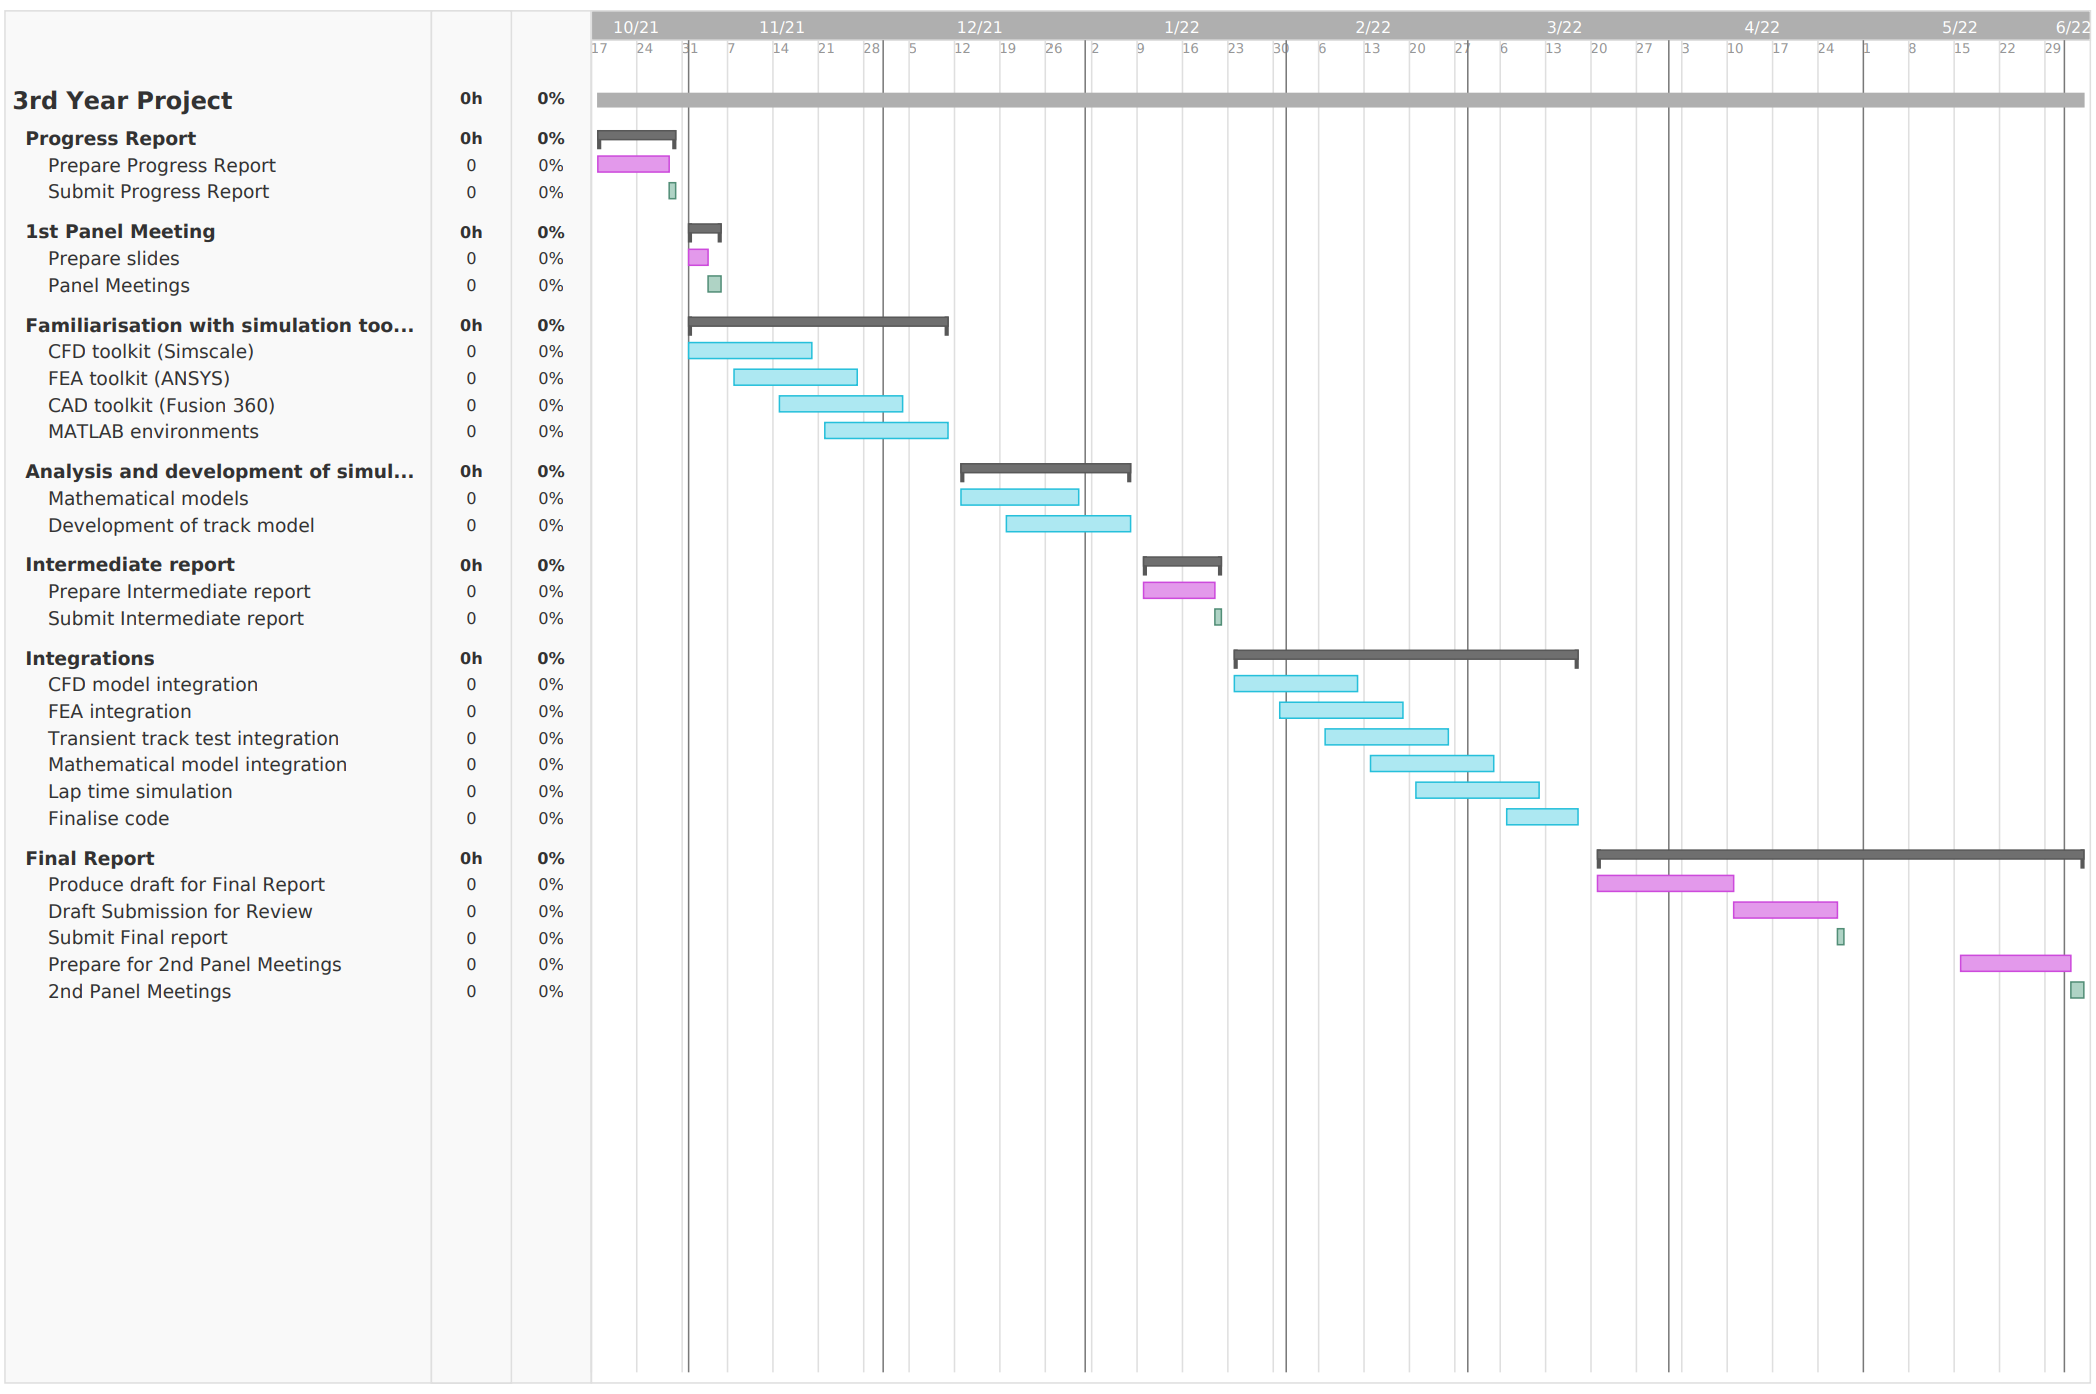
\includegraphics[width = 0.83 \textwidth]{./img/GanttChartProgressReport.png}
	\caption{Gantt Chart for the project.}
\end{figure}


\bibliographystyle{agsm}
\bibliography{./bib/export}

%----------------------------------------------------------------------------------------

\end{document}
